\chapter{Background}
\section{Machine Learning}

 Machine learning is a method of analyzing data in which a 
computer automatically iterates through large amounts of data 
without explicit programming to find patterns hidden in the data. 
The purpose of machine learning is to improve computer performance 
on a specific task over time through learning from data.
In other words, machine learning allows computers to adapt 
and improve performance on their own. 
Machine learning algorithms can be classified into two main 
categories: supervised learning and unsupervised learning. 

In Supervised learning, a model is trained on a labeled dataset,
which consists of input and corresponding output data. The model 
learns a function which maps the input data to the output data.
Once the model has learned this function, it can be used to make
predictions on unseen data, also known as out-of-sample data, 
that was not part of the original training dataset.
As an example, consider the task of predicting survival on the 
Titanic: the "Titanic - Machine Learning from Disaster" 
competition hosted by Kaggle\cite{titanic} requires participants 
to develop a model that accurately predicts whether an each person
on board survived the Titanic disaster or not. 
The model should be developed using the data in the training set.
The training set consists of information such as the gender and 
passenger ship class of each passenger on board and the results of 
whether the passenger survived or not.
The training set includes information about each passenger, such 
as their gender, age and ship class, and the outcome of whether 
they survived or not. This labeled data is used to build a machine
learning model that can predict whether they survived  based on 
other available information of the passengers.

In contrast to supervised learning models, which rely on labeled 
training data, unsupervised learning models do not use such data.
Since the goal of unsupervised learning is to find unknown patterns
that exist in the data, we only provide the input data to the model.
The model discovers regularities and features on its own, without
the guidance of labeled training data.

\begin{figure}[h]
  \centering
  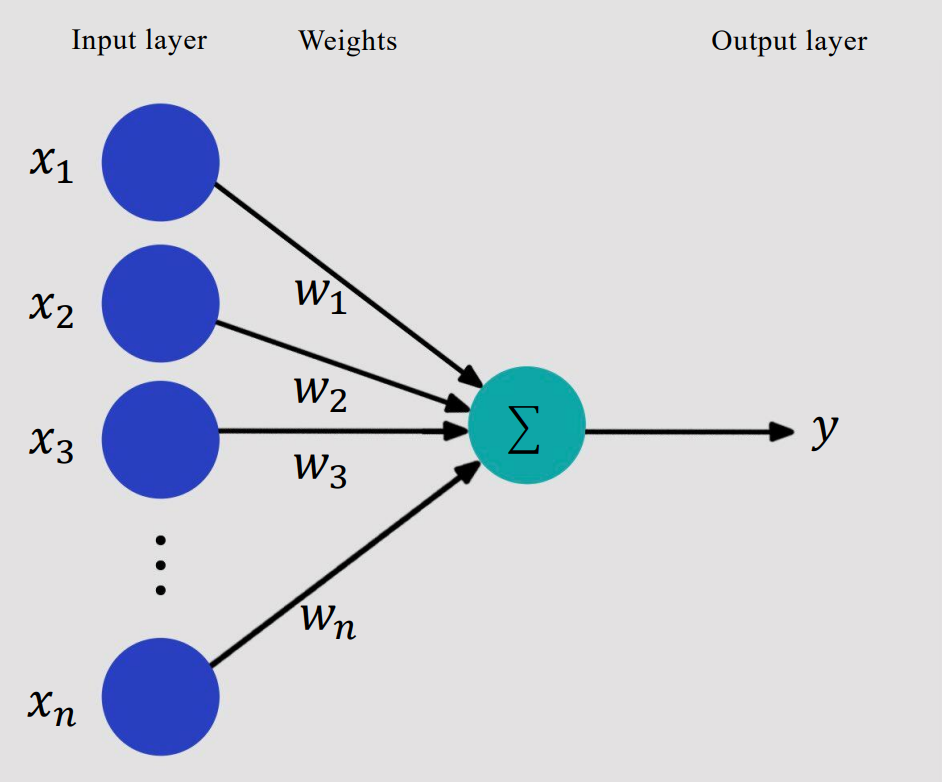
\includegraphics[width=130truemm]{resources/2_background/simple_perceptron.png}
  \caption{
    An example of simple perceptron
  }
  \label{simple_perceptron}
\end{figure}

\section{Neural Networks}
 Neural networks are a kind of machine learning algorithms which 
algorithm is modeled after the function and structure of human 
neural circuits and consist of a large number of interconnected 
processing nodes called neurons.
Frank Rosenblatt's simple perceptron \cite{Rosenblatt1958ThePA} was 
an early example of an artificial neural network. 
Simple perceptron consists of a single neuron that receives inputs 
from multiple sources and generates a single output. 
The structure of it is shown in Figure \ref{simple_perceptron}. 
The figure clearly shows how the perceptron processes received inputs.
The inputs $x_1, x_2 ... x_n$ are multiplied by their respective weights
$w_1, w_2 ... w_n$ and summed to produce the output $y$.
This can be expressed mathematically as follows:
\begin{equation}
  \label{perceptron_output}
  y = \sum_{k}w_k x_k + b
\end{equation}
where $b$ is a term called bias which is a variable that determines 
whether or not the output $y$ is set to 1.
During simple perceptron training, the goal is to find the optimal 
weights $w_1, w_2 ... w_n$, that will produce the correct output for 
a given set of inputs.
However, simple perceptrons are limited in its learning ability because 
they can only model linear relationships between inputs and outputs.
Therefore more complex neural networks are needed for learning tasks 
that require the modeling of nonlinear relationships.
A multilayer perceptron, which is a multilayer version of a simple 
perceptron, is one example. Figure \ref{multilayer_perceptron} shows
the most basic multilayer perceptron, which consists of three layers: 
an input layer, a hidden layer, and an output layer.

\begin{figure}[h]
  \centering
  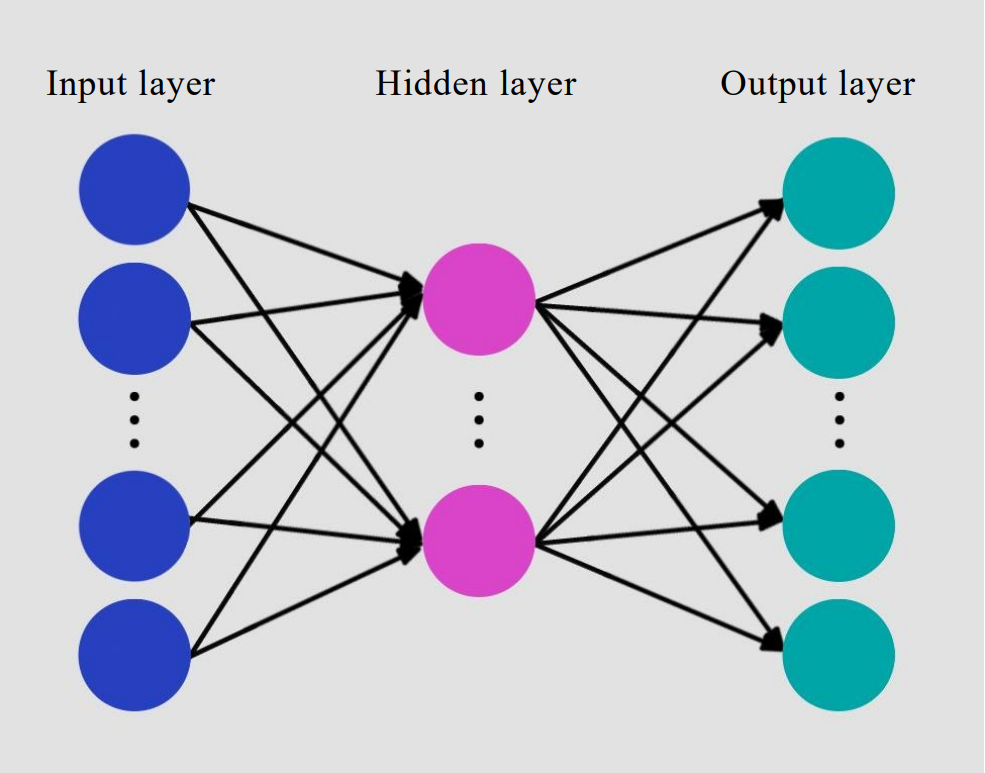
\includegraphics[width=130truemm]{resources/2_background/multi_layer_perceptron.png}
  \caption{
    An example of multi layer perceptron
  }
  \label{multilayer_perceptron}
\end{figure}
While Figure \ref{simple_perceptron} consists of an input layer and an 
output layer, Figure \ref{multilayer_perceptron} has an additional hidden 
layer. The addition of this hidden layer let the network capture nonlinear
relationships between input data and output data.

隠れ層を2対上にしたものもMLP。
多層パーセプトロンよりも隠れ層を増やせば、より複雑な関数が表現できるのでは?
で、ディープラーニングの導入。

\cite{dastres:hal-03349542}

\section{Deep Learning}
隠れ層を増やしたニューラルネットワーク。層が"深い"からDeep Learning。
ディープラーニングネットワークの画像。(これはあくまで基本形)
活性化関数につなげる方法が難しい~
【やっぱ活性化関数について単純パーセプトロンか多層パーセプトロンのとこで
説明するべきだったか。。。】

\section{Convolutional Neural Network}
画像データを対象とする場合に用いる。(通常のNNでも画像は適用できるが、
要素を縦一列にしないといけない。画像は縦横の位置情報が重要。一列に
してしまっては重要なデータが失われる。二次元のまま利用できるのが理想)
で、うまれたのがCNN。画像を二次元のまま入力に用いることができる。

畳み込みとかプーリング、全結合とかはここで説明する。

\section{Transformers}
あああああああああああ

\section{まだ何か必要だと思う} 
ああああああああああああ